
\documentclass[a4paper,11pt]{article}
\usepackage[utf8]{inputenc}
\usepackage[cyr]{aeguill}
\usepackage[margin=0.8in]{geometry}
\usepackage{xspace}
\usepackage{amsmath}
\usepackage[english,francais]{babel}
\usepackage{url}
\usepackage{algorithm}
\usepackage{algpseudocode}
\usepackage{xcolor}
\usepackage{listings} % pour le code
\usepackage{graphicx} % pour les figures
\usepackage{newclude}

% Redefinition de la commande \url pour pour l'utiliser dans un document en français
% sans avoir de problème avec les deux-points
% (voir http://perso.mines-albi.fr/~gaborit/latex/latex-in-french.html)
\let\urlorig\url
\renewcommand{\url}[1] {%
	\begin{otherlanguage}{english}\urlorig{#1}\end{otherlanguage}%
}
\renewcommand{\contentsname}{Sommaire} % si tableofcontents au début
\newcommand{\Numero}{\No}
\newcommand{\numero}{\no}


% Pour inclure joliment des scripts R
\lstset {
	language=R,
	basicstyle=\scriptsize\ttfamily,
	commentstyle=\ttfamily\color{gray},
	numbers=left,
	numberstyle=\ttfamily\color{gray}\footnotesize,
	stepnumber=1,
	numbersep=5pt,
	backgroundcolor=\color{white},
	showspaces=false,
	showstringspaces=false,
	showtabs=false,
	frame=single,
	tabsize=2,
	captionpos=b,
	breaklines=true,
	breakatwhitespace=false,
	title=\lstname,
	escapeinside={},
	keywordstyle={},
	morekeywords={}
}

\begin{document}

\title{Compte-rendu du TP \\``Evaluation empirique d'un programme''}
\author{Nom, prénom et parcours de chaque étudiant}
\date{\today}
\maketitle

\tableofcontents
\newpage

Vous devrez rendre ce rapport complété au format PDF exclusivement, en l'uploadant dans la colonne RenduTPEvalPerf de l'UE M2COM dans Tomuss (\url{http://tomuss.univ-lyon1.fr}), avant le 26 janvier à 23h59. N'envoyez pas d'email. Ne rendez pas le code source Latex. Ne rendez pas non plus d'autres fichiers (données brutes sous Excel, figures, code C, etc). Les figures pertinentes et les lignes de code que vous avez modifiées devront être incluses dans le rapport PDF. La taille maximale de ce rapport est de 15 pages.


\section{Présentation sommaire du programme à évaluer}

\subsection{Données à fournir en entrée}

On fournit, en entrée, un fichier texte venant d'un roman.
Ce fichier contient uniquement le texte du roman. Il ne doit pas avoir de numéro de page ou d'éléments qui ne sont pas liés au texte lui-même.

\subsection{Données fournies en sortie}

En sortie, nous obtenons un texte composé de $m$ mots (si possible) issus du texte d'entrée.
Le résultat est une texte qui donne l'illusion d'avoir été rédigé par une personne.
Cette illusion va être plus ou moins efficace en fonction du paramètre $k$.
Une valeur trop grande du paramètre $k$ va donner un texte identique au texte d'origine.

\subsection{Algorithme}

% Décrivez en français ce que vous avez compris de l'algorithme. Expliquez entre autres ce que représentent $n$, $m$, et $k$, et en quoi l'algorithme est stochastique. Vous pouvez en plus écrire l'algorithme sous forme de pseudocode (bonus). Voir  \url{https://en.wikibooks.org/wiki/LaTeX/Algorithms#Typesetting_using_the_algorithmic_package} pour plus d'informations.

L'algorithme découpe le texte d'entrée en mots et les trie.
L'algorithme va successivement trouver l'index du mot anciennement utilisé, jusqu'à ce qu'il n'y ait plus de mots disponibles ou jusqu'à ce qu'il ait atteint le nombre de mots de sortie désiré. Ensuite, il sélectionne un nouveau mot à partir de cet index, et pour terminer, il écrit ce mot dans la sortie désirée.


\begin{itemize}
	\item $n$ représente le nombre de mots mesurés dans le fichier d'entrée.
	\item $m$ représente le nombre de mots que l'on souhaite avoir en sortie.
	\item $k$ représente le nombre de mots par phrase.
\end{itemize}

L'algorithme est stochastique dans sa sélection des mots. Néanmoins, sa stochasticité peut être annulée par l'utilisation d'une mauvaise graine pour l'initialisation de la fonction d'aléatoire (srand).
\\ \\
Le pseudocode se trouve en annexe.

\section{Premières mesures du temps d'exécution}

\subsection{Paramètres utilisés dans toute cette section}
% Indiquez ici les valeurs de $m$ et $k$ avec lesquelles vous avez travaillé pour cette section. Indiquez également le ou les fichiers d'entrée utilisé(s) et la ou les valeur(s) de $n$ correspondantes. Indiquez également votre environnement de travail : système d'exploitation, compilateur (version), options de compilation, processeur, mémoire vive, etc. 

% ** PARAMETRES UTILISES
% ** FICHIER(S)
% [DONE] ** ENVIRONNEMENT DE TRAVAIL

\subsubsection{Paramètres}

Étant donné que les tests n'ont pas été réalisés avec les mêmes paramètres à chaque fois, ceux-ci seront indiqués.


\subsubsection{Environnement de travail}
\begin{table}[H]
	\centering
	\caption{Informations sur la machine utilisée}
	\label{tab:environnementTravail}
	\begin{tabular}{c|c}
		\toprule
		OS & Microsoft Windows 10 Professionnel 10.0.10240\\
		Processeur & Intel(R) Core(TM) i7-4702MQ CPU @ 2.20GHz 4 coeurs 8 processeurs logiques\\
		Memoire & 7.66GB DDR3\\
		Disque & 1TB HDD Toshiba MQ01ABD100\\
		Compilateur & gcc 4.8.1 (Windows 10)\\
		\bottomrule
	\end{tabular}
\end{table}

% Pour chacune des sous-sections suivantes, indiquez le nombre de runs effectués pour soutenir vos résultats.

\subsection{Mise en évidence de la stochasticité de l'algorithme}
% Montrez la variabilité obtenue dans les temps d'exécution en incluant un histogramme du temps CPU dans votre rapport (Figure \ref{fig:histo-variabilite}). Quantifiez cette variabilité en indiquant l'écart-type de ce temps d'exécution (sans oublier de préciser le nombre de runs sur lequel cet écart-type a été calculé). 

% \begin{figure}[htbp]
% 	\begin{center}
% 		% remplacez par votre figure 
% 		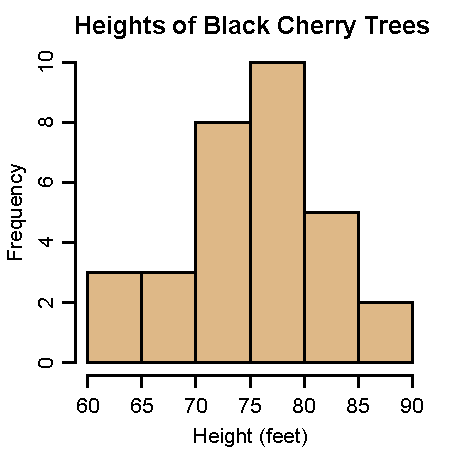
\includegraphics[width=6cm]{Black_cherry_tree_histogram.pdf}
% 		\caption{Black cherry tree histogram. Source: Wikimedia Commons.}
% 		\label{fig:histo-variabilite}
% 	\end{center}
% \end{figure}



% ** MONTRER VARIABILITE -> Histogramme

\begin{figure}[H]
	\begin{center}
		\includegraphics[height=8cm]{diagrams/time_m_10000_k_2.pdf}
		\caption{Mesure du temps CPU - m = 10000, k = 2}
		\label{fig:timeM10000K2}
	\end{center}
\end{figure}
Nous pouvons voir sur la figure \ref{fig:timeM10000K2} différents paliers représentant les différents fichiers d'entrée.
Chaque temps mesuré d'un palier (donc d'un fichier) est une exécution identique les unes par rapport aux autres.
Nous voyons donc qu'au sein d'un même palier, les temps varient, représentant la stochasticité de l'algorithme.

\begin{figure}[H]
	\begin{center}
		\includegraphics[height=8cm]{diagrams/time_m_100000_k_2.pdf}
		\caption{Mesure du temps CPU - m = 100000, k = 2}
		\label{fig:timeM100000K2}
	\end{center}
\end{figure}
Sur la figure \ref{fig:timeM100000K2}, nous pouvons voir une stochasticité plus importante, sûrement dû à une valeur de m 10 fois plus grande.

\begin{figure}[H]
	\begin{center}
		\includegraphics[height=7cm]{diagrams/time_m_100000_k_2_n_39213.pdf}
		\caption{Mesure du temps CPU - m = 100000, k = 2, n = 39213}
		\label{fig:timeM100000K2n39213}
	\end{center}
\end{figure}
La figure \ref{fig:timeM100000K2n39213} montre la stochasticité de l'algorithme sur un seul palier. Ceci veut dire que tous les points représentent le temps d'exécution avec des paramètres identiques.

% ** ECART-TYPE


\begin{table}[H]
	\centering
	\caption{Valeurs de $n$ choisies}
	\label{tab:ecartTypesTemps}
	\begin{tabular}{ccc|c}
		\toprule
		m & k & n & Ecart-type\\
		\midrule
		100000 & 2 & 39213 & 24.35136 ms\\
		100000 & 7 & 39213 & 31.43317 ms\\
		100000 & * & 39213 & 29.36821 ms\\
		\bottomrule
	\end{tabular}
\end{table}


% ** NB RUNS
Ces tests ont été réalisés en 10 runs.
\newline


% Puis décrivez la manipulation que vous avez effectuée pour montrer qu'une grande part de cette variabilité provient de la stochasticité de l'algorithme. 

Nous avons appliqué à $srand$ une valeur fixe (ici, 0). Ainsi, à chaque exécution de mêmes paramètres, les résultats seront très proches les uns des autres. Cela peut être clairement vu sur la figure \ref{fig:timeStochasticite}, avec, en noir, 100 exécutions avec une graine qui change, et en rouge, 100 exécutions avec une graine constante :

\begin{figure}[H]
	\begin{center}
		\includegraphics[height=7.6cm]{diagrams/time_serial_paral.pdf}
		\caption{Temps CPU - srand fixe}
		\label{fig:timeStochasticite}
	\end{center}
\end{figure}

\subsection{Influence de la charge système}
% En vous appuyant sur le cours, expliquez pourquoi le temps CPU, bien que fait pour être le plus indépendant possible de la charge système, peut tout de même être influencé par la charge système en pratique. Décrivez l'expérience que vous avez effectuée pour tester cet effet et synthétisez-en les résultats, en appuyant vos affirmations sur des chiffres. 

% ** PK TMPS CPU INFLUENCé PAR LA CHARGE SYSTEME?
Le temps CPU est influencé par la charge système car si celui-ci est très demandé par d'autres processus, alors il y a plus de chance pour que le processeur soit coupé entre deux mesures de temps pour donner la main à un autre processus.

% ** DECRIRE EXPERIENCE
Pour observer ce phénomène, il suffit de lancer les tests en série et de les comparer aux mêmes tests lancés en parallèle.
Étant donné que le système va devoir passer d'un processus à l'autre, nous observerons donc des différences.

% ** DONNER RESULTATS CHIFFRéS
100 tests ont été faits, avec comme paramètres k=3, m=100000 et, comme fichier, Le catéchumène (6640 mots).

Pour pouvoir observer en grande précision, les tests ont été faits en mesurant non pas le temps, mais un compteur incrémenté par le système (qui représente le temps lorsqu'il est divisé par la fréquence du processeur), ce qui a été fait pour être facilement analysable par des êtres humains.

\begin{table}[H]
	\centering
	\caption{Résultats}
	\label{tab:resultatTemps}
	\begin{tabular}{c|cc}
		\toprule
		& Série & Parallèle\\
		\midrule
		Écart-type & 0.005357606 & 0.02199298\\
		Minimum & 0.004862 & 0.007019\\
		Maximum & 0.031609 & 0.097435\\
		Moyenne & 0.00938539 & 0.0249153\\
		Médiane & 0.0075155 & 0.0155945\\
		\bottomrule
	\end{tabular}
\end{table}

\begin{figure}[H]
	\begin{center}
		\includegraphics[height=12cm]{diagrams/time_serial_paral.pdf}
		\caption{Temps d'exécution en parallèle}
		\label{fig:timeSerialParal}
	\end{center}
\end{figure}
En rouge, nous pouvons voir le temps d'exécution en parallèle.
En noir, nous pouvons voir le temps d'exécution en série.
Les lignes représentent les moyennes.


\subsection{Influence des options de compilation}
% Quantifiez le gain de performance obtenu en passant d'une compilation en mode debug à une compilation en mode release (option d'optimisation) : indiquez le pourcentage d'amélioration ainsi que la façon dont vous l'avez calculé (formule, mais aussi nombre de runs, etc).

% ** GAIN PERFORMANCE ENTRE DEBUG ET RELEASE

% Histogramme optimisation
% black = O0
% blue = O1
% orange = O2
% red = O3

\begin{figure}[H]
	\begin{center}
		\includegraphics[height=12cm]{diagrams/time_optimisation.pdf}
		\caption{Temps d'exécution en fonction de l'optimisation}
		\label{fig:timeOptimisation}
	\end{center}
\end{figure}

Nous pouvons constater sur la figure \ref{fig:timeOptimisation} que si l'optimisation n'a pas été activée (noir) ou si elle a été activée au niveau 1 (bleu), cela n'implique aucun changement de temps d'exécution. Mais à partir de l'optimisation de niveau 2 (orange), on constate une amélioration. L'optimisation de niveau 3 (rouge) n'implique aucune amélioration par rapport au niveau 2.


% ** % d'amélioration
% ** FORMULE
$moyenne(tempsDebug) = 0.00981731$
\par
$moyenne(tempsRelease) = 0.006638$
\par
$moyenne(tempsRelease) / moyenne(tempsDebug) = 0.6761526$
\par => Amélioration de 67.61526 \%

% ** NB RUNS, ...
Il y a eu 100 runs pour chaque paramètre d'optimisation, avec pour paramètres k=3, m=100000 et, comme fichier, Le catéchumène (6640 mots).
Les optimisations sont : 0, 1, 2, 3



\section{Opération dominante}

\subsection{Paramètres utilisés dans toute cette section}

\subsection{Identification de l'opération dominante}
Indiquez le ou les outils de profilage utilisés pour trouver l'opération dominante. Pour appuyer votre réponse, vous pouvez copier-coller un extrait du rapport de profilage, ou inclure une capture d'écran comme figure.

\subsection{Comptage des appels à l'opération dominante}
Indiquez ici les lignes de code que vous avez modifiées pour compter les appels à l'opération dominante.

\begin{lstlisting}[language=C]
/* A remplacer par les passages que vous avez modifies */
int i = 0;
float v = 5.9;
\end{lstlisting}



\section{Analyse de l'expérience fournie par R. Thion}

Rappelez le ou les objectifs de cette expérience (voir la partie 4 du sujet de TP) : à quelle(s) question(s) va-t-on répondre ?

\subsection{Plan d'expérience}
Rappelez ici le plan de l'expérience qui vous a été fournie :
\begin{itemize}
	\item Variables mesurées
	\item Paramètres que l'on a fait varier, et les valeurs choisies (sans oublier les fichiers d'entrée).
	\item Mode de combinaison des valeurs de paramètres (par exemple : full factorial design, si toutes les combinaisons possibles ont été testées)
	\item Nombre de runs effectués pour chaque combinaison de valeurs de paramètre
	\item Environnement de test
\end{itemize}

\subsection{Analyse des résultats}
Synthétisez les résultats obtenus à l'aide de trois figures maximum. Commentez-les et indiquez dans le texte principal les coefficients de détermination des régressions linéaires ($R^2$), les coefficients de corrélation et leurs p-values, etc.  Concluez sur les questions posées au début de cette section.



\section{Conception et réalisation de notre expérience}
% Indiquez ici le ou les objectifs de votre propre expérience (voir la partie 4 du sujet de TP, éventuellement enrichie de vos propres questions additionnelles).
Nous souhaitons tester l'influence de $n$, $m$ et $k$ sur les valeurs de $count1$, $count2$ et $count3$.

\subsection{Plan d'expérience}
% Décrivez ici votre plan d'expérience :
% \begin{itemize}
% 	\item Variables mesurées
% 	\item Paramètres que vous avez fait varier, et les valeurs choisies (justifiez). On peut considérer ici que les fichiers d'entrée font partie des paramètres, donc inpliquez lesquels vous avez choisis et expliquez pourquoi.
% 	\item Mode de combinaison des valeurs de paramètres (par exemple : full factorial design, si toutes les combinaisons possibles ont été testées)
% 	\item Nombre de runs effectués pour chaque combinaison de valeurs de paramètre
% 	\item Environnement de test
% \end{itemize}

% Si vous avez utilisé un outil de type ``cahier de laboratoire'' (papier ou numérique), indiquez-le ici, en incluant une figure (scan ou copie d'écran).

Pour réaliser les expériences et éviter le problème présenté dans l'analyse des résultats de l'expérience fournie vis à vis de l'initialisation de l'algorithme de génération de nombres aléatoires, nous avons utilisé une fonction de la librairie $windows.h$ qui retournera une valeur différente à chaque appel.

\begin{lstlisting}[language=C]
#include <windows.h>

/* [...] */

unsigned __int64 rndSeed;
QueryPerformanceCounter((LARGE_INTEGER *)&rndSeed);
srand(rndSeed);

/* [...] */
\end{lstlisting}


\subsubsection{Variables mesurées}

Les variables mesurées sont les suivantes :

\begin{table}[h!]
	\centering
	\caption{Variables mesurées}
	\label{tab:variablesMesureesExperience}
	\begin{tabular}{c|c}
		\toprule
		Variable & Description\\
		\midrule
		count1 & Nombre d'appels à la méthode $wordncmp$\\
		count2 & Nombre d'appels à la méthode $wordncmp$\\
		count3 & Nombre d'appels à la méthode $wordncmp$\\
		usr & Temps approximatif utilisé par le programme en lui même\\
		sys & Temps approximatif utilisé par le système d'exploitation\\
		time & Temps approximatif entre le début et la fin de l'exécution du programme\\
		\bottomrule
	\end{tabular}
\end{table}

\subsubsection{Paramètres}
Il a été réalisé 10 tests par jeu de paramètre.

\begin{table}[h!]
	\centering
	\caption{Paramètres numériques}
	\label{tab:parametresNumeriquesRealisee}
	\begin{tabular}{c|ccc}
		\toprule
		Paramètre & Valeur min & Valeur max & Incrément\\
		\midrule
		m & 100 & 1000000 & $*10$\\
		k & 2 & 7 & $+1$\\
		\bottomrule
	\end{tabular}
\end{table}

\begin{table}[h!]
	\centering
	\caption{Valeurs de $n$ choisies}
	\label{tab:valeursDeNChoisiesRealisee}
	\begin{tabular}{c|ccc}
		\toprule
		Fichier & Nombre de mots\\
		\midrule
		Le catéchumène & 6640\\
		Zig ou la destinée & 26046\\
		Venus Boy & 39213\\
		Battlefields of the Marne & 75166\\
		Madame Bovary & 112451\\
		Don Quixote & 404461\\
		Histoire des salons de Paris & 492732\\
		\bottomrule
	\end{tabular}
\end{table}


\subsubsection{Mode de combinaison des valeurs}
Les tests ont été effectués à partir de plages de paramètres. Toutes les valeurs possibles n'ont pas été utilisées, étant donné que certaines valeurs (par exemple : de grandes valeurs de $k$) ne sont plus adaptées à une utilisation cohérente du programme. C'est à dire que l'utilisation de tels paramètres donnerait un résultat d'exploitation (et non en terme de temps, etc...) non désiré dans une utilisation normale du programme.

\subsubsection{Nombre de runs}
Nous avons réalisé 2100 runs.

\subsubsection{Environnement de test}
\begin{table}[h!]
	\centering
	\caption{Informations sur la machine utilisée}
	\label{tab:environnementExperience}
	\begin{tabular}{c|c}
		\toprule
		OS & Microsoft Windows 10 Professionnel 10.0.10240\\
		Processeur & Intel(R) Core(TM) i7-4702MQ CPU @ 2.20GHz 4 coeurs 8 processeurs logiques\\
		Memoire & 7.66GB DDR3\\
		Disque & 1TB HDD Toshiba MQ01ABD100\\
		Compilateur & gcc 4.8.1 (Windows 10)\\
		\bottomrule
	\end{tabular}
\end{table}


\subsection{Analyse des résultats}
% Synthétisez les résultats obtenus à l'aide de trois figures maximum, et commentez-les. Les relations obtenues correspondent-elles à ce qu'on attend étant donné l'algorithme ? Quelle est l'influence de chaque paramètre ? Obtenez-vous les mêmes résultats qu'avec l'expérience fournie ?


Count1 $\sim$ n + k + m
\begin{verbatim}
Estimate Std. Error t value Pr(>|t|)    
(Intercept) -6.856e+05  2.629e+05  -2.608  0.00917 ** 
n            1.209e+01  4.757e-01  25.421  < 2e-16 ***
k            7.583e+04  5.109e+04   1.484  0.13789    
m            1.718e-02  2.233e-03   7.694 2.18e-14 ***
\end{verbatim}
Nous pouvons voir que seul n est fortement lié à Count1.\\
$R^2$ de $count1$ $\sim$ $n$ : 0.2301\\

Count2 $\sim$ n + k + m
\begin{verbatim}
Estimate Std. Error t value Pr(>|t|)    
(Intercept) -2.753e+05  7.855e+03  -35.05   <2e-16 ***
n            2.247e+01  1.422e-02 1580.88   <2e-16 ***
k            1.853e+04  1.527e+03   12.14   <2e-16 ***
m            4.283e-17  6.673e-05    0.00        1    
\end{verbatim}
Nous pouvons voir que seul n et k sont fortement liés à Count2.\\
$R^2$ de $count2$ $\sim$ $n$ : 0.9991\\
$R^2$ de $count2$ $\sim$ $k$ : -0.0004177\\

Count3 $\sim$ n + k + m
\begin{verbatim}
Estimate Std. Error t value Pr(>|t|)    
(Intercept)  3.356e+06  3.457e+05   9.708  < 2e-16 ***
n            8.389e+00  6.256e-01  13.409  < 2e-16 ***
k           -8.403e+05  6.719e+04 -12.506  < 2e-16 ***
m            1.241e-02  2.937e-03   4.225 2.49e-05 ***
\end{verbatim}
Nous pouvons voir que n et k sont étroitement liés à Count3.\\
$R^2$ de $count3$ $\sim$ $n$ : 0.07295\\
$R^2$ de $count3$ $\sim$ $k$ : 0.06339\\

Coefficients de corrélation :
\begin{verbatim}
count1        count2      count3
n 0.48010732  9.995515e-01  0.27090054
k 0.02803182  7.675098e-03 -0.25266565
m 0.14530334 -2.633931e-20  0.08536216
\end{verbatim}


Nous n'obtenons pas les mêmes résultats que l'expérience fournie. Cela peut venir de la stochasticité du programme, du problème d'initialisation de l'algorithme aléatoire pour l'expérience fournie et/ou des fichiers utilisés qui peuvent avoir des caractéristiques particulières.


\section{Annexe : Code réalisé pour le tutoriel sur les tests d'hypothèse}
\begin{algorithm}[H]
	\caption{Algorithme du générateur de texte.}
	\label{algoGeneTexte}
	\begin{algorithmic}
		\State $nword\gets splitInputIntoWords(word)$ \Comment {Découper le fichier d'entrée en mots}
		\State $sort(word)$
		
		\State $phrase\gets inputchars$
		\State $wordsleft\gets m$
		
		\For {$wordsleft > 0$} \Comment {Jusqu'à ce que l'on ait tous les mots que nous voulions.}
		
		\Comment {Dichotomie pour trouver l'index du mot qui correspond le mieux à $phrase$.}
		\State $lo\gets -1$ \Comment {Début du tableau de mots d'entrée.}
		\State $up\gets nword$ \Comment {Fin du tableau de mots d'entrée.}
		\While {$lo + 1 \neq up$}
		\State $mid\gets (lo + up) / 2$ \Comment {mid = médiane entre $lo$ et $up$.}
		\If {$isSmallerThan(word[mid], phrase)$}
		\State $lo\gets mid$
		\Else
		\State $up\gets mid$
		\EndIf
		\EndWhile
		
		
		\State $i\gets 0$
		\For {$phrase = word[up + i]$}
		\If {!(rand() \% (i + 1))} \Comment {Se produit de moins en moins souvent au fur et à mesure que la valeur de i augmente.}
		\State $p\gets word[up + i]$
		\EndIf
		\State $i\gets i + 1$
		\EndFor
		
		\State $phrase\gets skip(p, 1)$ \Comment {Sélectionne le mot choisi aléatoirement.}
		\If {isEmptyString(skip(phrase, k-1))} \Comment {Si nous avons atteint la fin du fichier.}
		\State $break$ \Comment {Quitte la boucle.}
		\EndIf
		
		\State $writeOutputWord(skip(phrase, k-1))$
		
		\State $wordleft\gets wordleft - 1$ \Comment {Décompte le nombre restant de mots à ajouter au texte final.}
		\EndFor
		
	\end{algorithmic}
\end{algorithm}
\newpage
\begin{lstlisting}[language=R]
#######################
# Cas ou H0 est vraie 
####################### 

# On va considerer deux populations qui ont exactement
# les memes parametres : les deux sont uniformement 
# distribuees entre 0 et 1. Les deux populations ont
# donc la meme moyenne, en l'occurrence 0.5. 
# Puis nous allons faire une experience : 
# - tirer un petit echantillon dans chaque population
# - calculer la moyenne observee dans l'echantillon 1,
#   puis celle observee dans l'echantillon 2. On 
#   n'obtiendra pas exactement 0.5 ni pour l'une ni pour 
#   l'autre.
# - calculer la difference entre les deux moyennes 
#   d'echantillons. Appelons d cette difference.

tirerEchantillonPop1H0 <- function(n) {
	vraieMoyenne <- 0.5
	plageDeDispersion <- 1.0
	min <- vraieMoyenne - plageDeDispersion/2.0
	max <- vraieMoyenne + plageDeDispersion/2.0
	ech <- runif(n, min, max)
	return(ech)
}

tirerEchantillonPop2H0 <- function(n) {
	vraieMoyenne <- 0.5
	plageDeDispersion <- 1.0
	min <- vraieMoyenne - plageDeDispersion/2.0
	max <- vraieMoyenne + plageDeDispersion/2.0
	ech <- runif(n, min, max)
	return(ech)
}

# Ecrire ici le code permettant de faire une "experience"
# c'est a dire tirer un echantillon de taille 20 dans 
# chaque population et mesurer la difference d observee
# entre les 2 moyennes d'echantillon.
pop1 <- tirerEchantillonPop1H0(20)
pop2 <- tirerEchantillonPop2H0(20)

mean(pop1)
mean(pop2)
abs(mean(pop1) - mean(pop2))
abs(mean(tirerEchantillonPop1H0(20)) - mean(tirerEchantillonPop2H0(20)))

# Si 1000 etudiants font independamment cette experience,
# chaque etudiant aura des echantillons differents et donc
# chacun aura une valeur differente pour d. Si nous 
# mettons toutes ces 1000 valeurs ensemble dans un vecteur
# (appele diffMoyH0), quelle sera la moyenne de ce vecteur ?

diffMoyH0 = c()

for(i in  1:1000)
{
	diffMoyH0 = c(diffMoyH0, abs(mean(tirerEchantillonPop1H0(20)) - mean(tirerEchantillonPop2H0(20))))
}

# On affiche la moyenne totale.
mean(diffMoyH0)

# On affiche les 1000 valeurs sur un histogramme.
plot(diffMoyH0)
abline(h=mean(diffMoyH0), col="red")

\end{lstlisting}

Nous obtenons une moyenne de 0,07.
\newpage
\begin{lstlisting}[language=R]

#######################
# Cas ou H1 est vraie 
####################### 

# On va voir comment se comporte notre indicateur quand 
# les deux populations n'ont pas la meme moyenne
# (mais ont tout de meme la meme dispersion)
# eg . pop1 comprise entre 0.0 et 1.0
#   et pop2 comprise entre 0.2 et 1.2 

tirerEchantillonPop1H1 <- function(n) {
	vraieMoyenne <- 0.5
	plageDeDispersion <- 1.0
	min <- vraieMoyenne - plageDeDispersion/2.0
	max <- vraieMoyenne + plageDeDispersion/2.0
	ech <- runif(n, min, max)
	return(ech)
}

tirerEchantillonPop2H1 <- function(n) {
	vraieMoyenne <- 0.7
	plageDeDispersion <- 1.0
	min <- vraieMoyenne - plageDeDispersion/2.0
	max <- vraieMoyenne + plageDeDispersion/2.0
	ech <- runif(n, min, max)
	return(ech)
}


# Ecrire ici le code pour faire les 1000 experiences 
# comme precedemment, en nommant cette fois le vecteur
# diffMoyH1. Calculez sa moyenne et tracez son histogramme.

diffMoyH1 = c()

for(i in  1:1000)
{
	diffMoyH1 = c(diffMoyH1, abs(mean(tirerEchantillonPop1H1(20)) - mean(tirerEchantillonPop2H1(20))))
}

# On affiche la moyenne totale.
mean(diffMoyH1)

# On affiche les 1000 valeurs sur un histogramme.
plot(diffMoyH1)
abline(h=mean(diffMoyH1), col="red")

\end{lstlisting}

Nous obtenons une moyenne de 0,2.

\begin{figure}[H]
	\begin{center}
		% remplacez par votre figure 
		\includegraphics[width=10cm]{diagrams/diffMoy.pdf}
		\caption{Graphique représentant diffMoyH0 et diffMoyH1 ainsi que leur moyenne}
		\label{fig:diffMoy}
	\end{center}
\end{figure}


Plaçons nous maintenant dans le cas où l'on ait fait une seule expériencee.

% Ecrire le code pour evaluer la plausibilite de H0: "les deux echantillons proviennent de deux populations qui ont la meme moyenne".

\begin{lstlisting}[language=R]
cMean <- function(v1, v2)
{
	return(abs(mean(v1) - mean(v2)))
}
sameMean <- function(v1, v2)
{
	return(cMean(v1, v2) < 0.1)
}

sameMean(tirerEchantillonPop1H0(20), tirerEchantillonPop2H0(20))
sameMean(tirerEchantillonPop1H1(20), tirerEchantillonPop2H1(20))

x1 <- c(0.97050525, 0.13734516, 0.80793033, 0.05207726, 0.62629180, 0.93485856,
0.58220744, 0.65935145, 0.76467195, 0.73512414, 0.45139560, 0.93225380,
0.53790595, 0.99845675, 0.31035081, 0.43082815, 0.15475353, 0.42647652,
0.65676067, 0.74186048)
x2 <- c(0.33565036, 0.28830545, 0.51556544, 0.93223089, 0.29192576, 0.43505823,
0.63127002, 0.86082799, 0.56533392, 0.19083212, 0.13087779, 0.09849703,
0.98921291, 0.91480756, 0.78556552, 0.33859160, 0.88482223, 0.76701274,
0.24190609, 0.46251866)

cMean(x1, x2)
sameMean(x1, x2)
\end{lstlisting}

Ici, sameMean(x1, x2) retourne "TRUE", ce qui signifie que les deux échantillons ont une moyenne proche l'une de l'autre.

\begin{figure}[H]
	\begin{center}
		% remplacez par votre figure 
		\includegraphics[width=7cm]{diagrams/x1-x2-1.pdf}
		\caption{Graphique représentant x1 and x2 ainsi que leur moyenne}
		\label{fig:x1-x2-1}
	\end{center}
\end{figure}

\begin{lstlisting}[language=R]
x1 <- c(0.41236444, 0.28422821, 0.15093798, 0.05885328, 0.25514435, 0.63026931,
0.56325462, 0.76304859, 0.56523993, 0.92535660, 0.10898729, 0.51579642,
0.07223967, 0.53483839, 0.52516575, 0.20250815, 0.89634680, 0.53879059,
0.58736912, 0.53945749)
x2 <- c(1.0809923, 0.5772333, 0.7252340, 1.1529082, 1.0924642, 0.6046166, 0.9495800,
0.3019857, 0.7701195, 1.0746508, 0.3928894, 1.0885017, 0.5101510, 1.1871599,
0.7953318, 0.5711237, 0.5505642, 0.9854085, 0.5105643, 0.9601635)

cMean(x1, x2)
sameMean(x1, x2)
\end{lstlisting}

Ici, sameMean(x1, x2) retourne "FALSE", ce qui signifie que les deux échantillons ont une moyenne bien différente l'une de l'autre.

\begin{figure}[H]
	\begin{center}
		\includegraphics[width=7cm]{diagrams/x1-x2-2.pdf}
		\caption{Graphique représentant x1 and x2 ainsi que leur moyenne}
		\label{fig:x1-x2-2}
	\end{center}
\end{figure}


%Incorporez également les histogrammes obtenus sous forme de figures. Indiquez vos conclusions sur les deux paires d'échantillons. 



\end{document}